\documentclass[12pt]{article}
\usepackage{graphicx}
\usepackage[utf8]{inputenc}
\usepackage{geometry}
\geometry{a4paper, margin=0.75in}
\usepackage{titlesec}
\usepackage{enumitem}
\usepackage{hyperref} 
\usepackage{amsmath}
\usepackage{ gensymb }
\usepackage{ amssymb }
\usepackage{float}
\usepackage{amsthm}
\usepackage{float}
\usepackage{enumitem}
\usepackage{pgfplots}

\newcommand{\st}{\text{s.t}}

\title{PSET1}
\author{Anthony Yoon}
\date{1/8/2025}
\begin{document}
\maketitle
\section*{Q1}
\subsection*{a}
\begin{align*}
    \max & \quad x^\alpha_1 x_2^{1-\alpha}\\
    \st & \quad p_1 x_1 + p_2 x_2 \leq m \\
    & \quad x_1 \geq 0, x_2 \geq 0 
\end{align*}
\subsection*{b}
The Langrangian is 
\[
L =  x^\alpha_1 x_2^{1-\alpha} - \lambda(m - p_1x_1 + p_2 x_2)
\]
and the Kuhn Tucker first order conditions are
\begin{align*}
    [x_1] & \quad \alpha \left( \frac{x_2}{x_1} \right)^{1-\alpha} \leq \lambda p_1 \text{ and } x_1 \geq 0\\
    [x_2] & \quad (1-\alpha) \left( \frac{x_1}{x_2} \right)^{\alpha} \leq \lambda p_2 \text{ and } x_2 \geq 0\\
    [\lambda] & \quad m = p_1 x_1 + p_2 x_2
\end{align*}
\subsection*{c}
Note that note that if $x_1 = x_2 = 0$, than the first order conditions become undefined. Thus, $x_1 > 0$ and $x_2 > 0$. Therefore, by complemntary slackness, we see that 
\[
    \alpha \left( \frac{x_2}{x_1} \right)^{1-\alpha} = \lambda p_1 \quad (1-\alpha) \left( \frac{x_1}{x_2} \right)^{\alpha} = \lambda p_2
\]
Therefore, we see that when we equate $\lambda$s, we see that 
\[
 \frac{\alpha}{1-\alpha} \left( \frac{x_2}{x_1} \right) = \frac{p_1}{p_2}
\]
\[
\frac{\alpha}{1-\alpha} \left( p_2x_2 \right) = p_1 x_1
\]
Thus, we can see that 
\[
m = \frac{\alpha}{1-\alpha} p_2 x_2 + p_2 x_2
\]
\[
m = \frac{p_2 x_2}{1-\alpha} 
\]
\[
\frac{m(1-\alpha)}{p_2} = x_2^*
\]
Similarly, we can find that 
\[
x_1^* = \frac{\alpha m}{p_1}
\]
\subsection*{d}
Note
\[
x_1^* p_1 = \alpha m \quad x_2^* p_2 = (1-\alpha)m
\]
So the optimal expenditures are not reliant on price, so when $p_1$ increases, then both optimal expenditures are not affected. 
\subsection*{e}
\[
V(p_1,p_2,m) = \left(  \frac{\alpha m}{p_1} \right)^{\alpha} \left( \frac{m(1-\alpha)}{p_2}\right)^{1-\alpha}
\]
\subsection*{f}
Note that in the derivation of the Marshallian demand functions, we have the following expression. 
\[
    \frac{\alpha}{1-\alpha} \left( \frac{x_2}{x_1} \right) = \frac{p_1}{p_2}
\]
And if we multiply prices by some constant factor, that factor would get canceled out, as $k / k = 1$ Thus, $x_i(p_1,p_2,m)^*$ is homogenous in degree 0. 
\subsection*{g}
$V(p_1,p_2,m)$ is dependent on $x_i^*$. And thus, if $x^*_i$ changes due to a change in prices, then logically speaking, than $V(p_1, p_2, m)$ would change as well. However, since $x_i^*$ is homogenous in degree 0, that means that it does not change in response to a change in prices, which means that $V(p_1,p_2,m)$ does not do so as well. Thus, $V(p_1,p_2,m)$ is homogenous in degree 0.
\subsection*{h}
The economic intuition is that individuals with a Cobbs Douglas utility function will only allocate a certain percentange of their income (deonted by $\alpha$), and thus does not respond to a change in prices.
\subsection*{i}
\[
\frac{\partial V}{\partial m} = \left( \frac{\alpha}{p_1} \right)^{\alpha} \left( \frac{1-\alpha}{p_2} \right)^{1-\alpha}
\]
\subsection*{j}
Note that Roy's identity is 
\[
x_i(p_1, p_2, m) = -\frac{\frac{\partial V}{\partial p_i}}{\frac{\partial V}{\partial m}}
\]
Rearranging the terms yields:
\[
- x_i \cdot \frac{\partial V}{\partial m} = \frac{\partial V}{\partial p_i}
\]
And we can see that 
\[
\frac{\partial V}{\partial m} = \left( \frac{\alpha}{p_1} \right)^{\alpha} \left( \frac{1-\alpha}{p_2} \right)^{1-\alpha}
\]
Thus, for $i = 1$, we see that
\[
    -\frac{\alpha m}{p_1} *  \left( \frac{\alpha}{p_1} \right)^{\alpha} \left( \frac{1-\alpha}{p_2} \right)^{1-\alpha} = \frac{\partial V}{\partial p_1}
\]
And similarly 
\[
- \frac{(1-\alpha)m}{p_2} *  \left( \frac{\alpha}{p_1} \right)^{\alpha} \left( \frac{1-\alpha}{p_2} \right)^{1-\alpha} = \frac{\partial V}{\partial p_2}
\]
\subsection*{k}
(i) and (j) are related because the marginal utility of price is inversely proportional to the marginal utility of income. So if the marginal utilty of income increases, then the marginal utilty of price will down. 
\section*{Q2}
\subsection*{a}
The Langrangian is 
\[
L = \alpha \ln(x_1) + (1-\alpha) \ln(x_2) - \lambda(m-p_1x_1 - p_2x_2)
\]
and the according the first order conditions are:
\begin{align*}
    [x_1] & \quad \frac{\alpha}{x_1} \leq \lambda p_1 \text{ and } x_1 \geq 0\\
    [x_2] & \quad \frac{1-\alpha}{x_2} \leq \lambda p_2 \text{ and } x_2 \geq 0\\
    [\lambda] & \quad m = p_1 x_1 + p_2 x_2
\end{align*}
We can note that $x_1 \neq 0$ and $x_2 \neq 0$, as if this was the case, we can see that the first order conditions would not hold. Therefore, by complemntary slackness, we know that $x_1 > 0$ and $x_2 > 0$, which implies that $[x_1]$ and $[x_2]$ must be strict equalities. Therefore, we can equate the equalities via the $\lambda$s, where we get 
\[
\frac{\alpha}{x_1 p_1} = \frac{1-\alpha}{x_2 p_2}
\]
\[
\frac{\alpha}{1-\alpha} = \frac{x_1 p_1}{x_2p_2}
\]
\[
x_2p_2 \left( \frac{\alpha}{1-\alpha} \right) = x_1p_1
\]
And we use this in conjunction with the $[\lambda]$ condition. We can see that 
\[
x_2 p_2 + x_2p_2 \left( \frac{\alpha}{1-\alpha} \right) = m \iff x_2 = \frac{m (1-\alpha)}{p_2}
\]
and similarly, 
\[
x_1p_1 + x_1p_1 \left( \frac{1-\alpha}{\alpha} \right) = m \iff x_1 = \frac{\alpha m }{p_1}
\]
and 
\[
V(p_1, p_2, m) = \alpha \ln\left(\frac{m \alpha}{p_1}\right) + (1-\alpha) \ln\left(\frac{m(1-\alpha)}{p_2}\right)
\]
Now, we can begin an analysis of how the answers from (1) change.  
\subsubsection*{How the answers change}
\begin{enumerate}[label=\alph*]
    \item Omitted, done above
    \item Omitted, done above
    \item Omitted, done above
    \item Omitted, done above
    \item 
    \[
    p_1 x_1^* = \frac{\alpha m}{p_1} * p_1 = \alpha m 
    \]
    \[
    p_2 x_2^* = \frac{(1-\alpha)m}{p_2} * p_2 = (1-\alpha) m 
    \]
    Thus, the answer does not change.
    \item The answer does not change here. Note that in the derivation of the Marshallian demand functions, we can see that we get the expression
    \[
\frac{\alpha}{1-\alpha} = \frac{x_1 p_1}{x_2p_2}
    \]
    where we can see that we can follow a similar logic in (1) to state that the multiplication of scalars to the price does not do anything.
    \item A similar logic from (1) can be used here. Since both Marshallian demand functions are homogenous in degree 0, then the indirect utility function must be homogenous in degree 0
    \item Answer does not change from (1), as the individual will only allocate a certain portion of their income towards the consumption of a good. 
    \item \begin{align*}
        V(p_1, p_2, m) &= \alpha \ln\left(\frac{m \alpha}{p_1}\right) + (1-\alpha) \ln\left(\frac{m(1-\alpha)}{p_2}\right)\\
        &= \alpha \left( \ln(m) + \ln \left( \frac{\alpha}{p_1} \right) \right) + (1-\alpha)\left( \ln(m) + \ln \left( \frac{1-\alpha}{p_2} \right) \right)\\
        &= \alpha \ln(m) + \alpha \ln \left( \frac{\alpha}{p_1} \right) + (1-\alpha) \ln(m) + (1-\alpha) \ln \left( \frac{1-\alpha}{p_2} \right)\\
        &= \ln(m) +  \alpha \ln \left( \frac{\alpha}{p_1} \right) + (1-\alpha) \ln \left( \frac{1-\alpha}{p_2} \right)
    \end{align*}
    Thus, 
    \[
    \frac{\partial V}{\partial m} = \frac{1}{m}
    \]
    \item We can use a similar process as in (1). We can see that roy's identity allows us to get the following expression
    \[
        - x_i \cdot \frac{\partial V}{\partial m} = \frac{\partial V}{\partial p_i}
    \]
    and thus we see that 
    \[
    \frac{\alpha m}{p_1} * \frac{1}{m} = \frac{\alpha}{p_1} = \frac{\partial V}{\partial p_1}
    \]
    and 
    \[
    \frac{(1-\alpha)m }{p_1} * \frac{1}{m} = \frac{1-\alpha}{p_2} = \frac{\partial V}{\partial p_2}
    \]
    \item They are not related \textbf{Not sure}
\end{enumerate}
\subsection*{b}
We are left with the following:
\begin{align*}
    \max & \quad x_1^\alpha x_2^\beta\\
    \st & \quad p_1 x_1 + p_2 x_2 \leq m 
\end{align*}
Using a simialr logic to above, we find that the first order conditions are
\begin{align*}
    [x_1] & \quad \alpha x^{\alpha - 1}_1 x_2^\beta = \lambda p_1\\
    [x_2] & \quad \beta x^\alpha_1 x_2^{\beta -1} = \lambda p_2\\
    [\lambda] & \quad p_1 x_1 + p_2 x_2 = m
\end{align*}
and equating the $\lambda$s yields 
\[
\frac{\alpha x_2}{\beta x_1} = \frac{p_1}{p_2} \iff \frac{\alpha p_2 x_2}{\beta} = p_1 x_1
\] 
and thus 
\begin{align*}
    p_1 x_1 + p_2 x_2 &= m \\
    p_2x_2\left( \frac{\alpha +\beta}{\beta}\right) &= m\\
    x_2 &= \frac{m \beta}{p_2(\alpha + \beta)}
\end{align*}
and by a similar logic, we can see that 
\[
x_1 = \frac{\alpha m}{p_1(\beta + \alpha)}
\]
The answers change in the following:
\subsubsection*{How the answers change}
\begin{enumerate}[label=\alph*]
    \item Shown above 
    \item Shown above 
    \item Shown above
    \item Shown above
    \item The answer does not change. Given how both Marshallian demand functions have the price in the denomintaor, multiplying the good by the price will cancle this term out, and thus leave cause the optimal expenditure on each good to be independent of any price change. 
    \item A similar logic can be seen as above. Note when we equate the $\lambda$s we see that prices are divided, so any scalar multiplication does not change the end Marshallian demand functions. 
    \item The answer does not change
    \item The economic intution here is that the consumer will only allocate a certain portion of their income on the consumption of a good. 
    \item Note that 
    \begin{align*}
        V(p_1, p_2, m) &= \left( \frac{\alpha m}{p_1(\beta + \alpha)} \right)^{\alpha} \left( \frac{\beta}{p_2(\alpha + \beta)} \right)^\beta \\
        &= m^{\alpha + \beta} \left( \frac{\alpha}{p_1(\alpha + \beta)} \right)^\alpha \left( \frac{\beta}{p_2(\alpha + \beta)} \right)^\beta
    \end{align*}
    Thus, 
    \begin{align*}
        \frac{\partial V}{\partial m} &= (\alpha + \beta) m^{\alpha + \beta -1} \left( \frac{\alpha}{p_1(\alpha + \beta)} \right)^\alpha \left( \frac{\beta}{p_2(\alpha + \beta)} \right)^\beta\\
        &= (\alpha + \beta)^{-\alpha - \beta + 1} m^{\alpha + \beta -1} \left( \frac{\alpha}{p_1} \right)^\alpha \left( \frac{\beta}{p_2} \right)^\beta
    \end{align*}
    \item We can use Roy's Identity to see that 
    \[
        - x_i \cdot \frac{\partial V}{\partial m} = \frac{\partial V}{\partial p_i}
    \]
    and thus
    \[
    -\frac{\alpha m}{p_1(\alpha + \beta)} \cdot (\alpha + \beta)^{-\alpha - \beta + 1} m^{\alpha + \beta -1} \left( \frac{\alpha}{p_1} \right)^\alpha \left( \frac{\beta}{p_2} \right)^\beta = \frac{\partial V}{\partial p_1}
    \]
    \[
    -(\alpha + \beta)^{-\alpha - \beta} m^{\alpha + \beta} \left( \frac{\alpha}{p_1} \right)^{\alpha + 1} \left( \frac{\beta}{p_2} \right)^\beta = \frac{\partial V}{\partial p_1}
    \]
    and by a similar logic we see that
    \[
        -(\alpha + \beta)^{-\alpha - \beta} m^{\alpha + \beta} \left( \frac{\alpha}{p_1} \right)^{\alpha} \left( \frac{\beta}{p_2} \right)^{\beta + 1} = \frac{\partial V}{\partial p_2}
    \]
    \item \textbf{TODO LATER}
\end{enumerate}
\subsection*{c}
Assume that now we are working with some arbitrary function that is
strictly concave and increasing in both $x_1$ and $x_2$. This ensures that there exists an optimal solution. 
\subsection*{How the answers change}
\begin{enumerate}[label=\alph*., start=6]
    \item We are not sure if the functions will stay homogenous in degree 0, as this condition only holds true for certain utility functions.
    \item We are not sure if the functions will stay homogenous in degree 0, as this condition only holds true for certain utility functions.
    \item We are not sure if the answer will stay the same or not because the economic intution for this is reliant on a consumer who allocates a proprotion of his income towards the expenditure of a good, regardless of price. 
    \item Since we use Roy's identity for this, we can always ensure that there exists some relation between the marginal utility of income at the optimal point and the margianl utilty of price at the optimal point
\end{enumerate}
\section*{Q3}
Now, we assume that the utility function is given by 
\[
u(x_1, x_2) = \left( \alpha x_1^{\frac{\sigma-1}{\sigma}} + (1-\alpha)x_2^{\frac{\sigma -1}{\sigma}} \right)^{\frac{\sigma}{\sigma -1}}
\]
\subsection*{a}
We begin by caclculating the MRS:
\begin{align*}
    \frac{\partial}{\partial x_1}\left( \alpha x_1^{\frac{\sigma-1}{\sigma}} + (1-\alpha)x_2^{\frac{\sigma -1}{\sigma}} \right)^{\frac{\sigma}{\sigma -1}} &= \left( \alpha x_1^{\frac{\sigma-1}{\sigma}} + (1-\alpha)x_2^{\frac{\sigma -1}{\sigma}} \right)^{\frac{\sigma}{\sigma -1} -1 } \cdot \alpha x_1^{-\frac{1}{\sigma}}\\
    \frac{\partial}{\partial x_2}\left( \alpha x_1^{\frac{\sigma-1}{\sigma}} + (1-\alpha)x_2^{\frac{\sigma -1}{\sigma}} \right)^{\frac{\sigma}{\sigma -1}} &= \left( \alpha x_1^{\frac{\sigma-1}{\sigma}} + (1-\alpha)x_2^{\frac{\sigma -1}{\sigma}} \right)^{\frac{\sigma}{\sigma -1} -1} \cdot (1-\alpha) x_2^{-\frac{1}{\sigma}}
\end{align*}
And thus, 
\[
\text{MRS} = \frac{\frac{\partial U}{\partial x_1}}{\frac{\partial U}{\partial x_2}} = \frac{\alpha}{1-\alpha} \cdot \left( \frac{x_2}{x_1} \right)^{\frac{1}{\sigma}} 
\]
Taking the natural log of this yields:
\[
\ln \left( \frac{\alpha}{1-\alpha} \cdot \left( \frac{x_2}{x_1} \right)^{\frac{1}{\sigma}} \right) = \ln \left( \frac{\alpha}{1-\alpha} \right) + \frac{1}{\sigma} \ln \left( \frac{x_2}{x_1} \right) 
\]
and note that 
\[
\frac{d \ln \left( \frac{x_2}{x_1} \right)}{d \ln(\text{MRS})} = \left( \frac{\ln (\text{MRS})}{\ln \left( \frac{x_2}{x_1} \right)} \right)^{-1}
\]
Thus, 
\[
\frac{d \ln \left( \frac{x_2}{x_1} \right)}{d \ln(\text{MRS})} = \left( \frac{\ln (\text{MRS})}{\ln \left( \frac{x_2}{x_1} \right)} \right)^{-1} = (\sigma^{-1})^{-1} = \sigma
\]
\qed
\subsection*{b}
Consider $\ln(u(x_1,x_2))$, as this will make calculations easier. We see that 
\[
\ln(u(x_1, x_2)) = \frac{\sigma}{\sigma - 1} \ln \left( \alpha x_1^{\frac{\sigma -1}{\sigma}} + (1-\alpha)x_2^{\frac{\sigma - 1}{\sigma}} \right)
\] 
We can clearly see that as $\sigma \to 1$, the function becomes undefined $(\frac{0}{0})$, as 
\[
\alpha x_1^{\frac{\sigma-1}{\sigma}} + (1-\alpha)x_2^{\frac{\sigma-1}{\sigma}} \to \alpha + 1-\alpha = 1
\]
We now differentiate both the numerator and denominator with respect to $\sigma$, getting that 
\begin{align*}
     & \frac{\partial }{\partial \sigma} \ln\left(\left( \alpha x_1^{\frac{\sigma -1}{\sigma}} + (1-\alpha)x_2^{\frac{\sigma - 1}{\sigma}} \right)^{\sigma}\right) \\
    &= \frac{\sigma \left( \alpha x_1^{\frac{\sigma -1}{\sigma}} + (1-\alpha)x_2^{\frac{\sigma - 1}{\sigma}} \right)^{\sigma - 1} \frac{\partial }{\partial \sigma} \left( \alpha x_1^{\frac{\sigma -1}{\sigma}} + (1-\alpha)x_2^{\frac{\sigma-1}{\sigma}}\right)}{\left( \alpha x_1^{\frac{\sigma -1}{\sigma}} + (1-\alpha)x_2^{\frac{\sigma - 1}{\sigma}} \right)}\\
    &= \frac{\sigma \frac{\partial }{\partial \sigma}\left( \alpha x_1^{\frac{\sigma -1}{\sigma}} + (1-\alpha)x_2^{\frac{\sigma - 1}{\sigma}} \right)}{\left( \alpha x_1^{\frac{\sigma -1}{\sigma}} + (1-\alpha)x_2^{\frac{\sigma - 1}{\sigma}} \right)^{\frac{\sigma - 1}{\sigma}}}
\end{align*}
 Next, we analyze the expression $\left( \alpha x_1^{\frac{\sigma -1}{\sigma}} + (1-\alpha)x_2^{\frac{\sigma - 1}{\sigma}} \right)$. As $\sigma \to 1$, we clearly see that $\frac{\sigma - 1}{\sigma} \to 0$. Therefore, 
\[
\lim_{\sigma \to 1} \left( \alpha x_1^{\frac{\sigma -1}{\sigma}} + (1-\alpha)x_2^{\frac{\sigma - 1}{\sigma}} \right) = 1
\]
 The denominator obviously appraoches 1 as $\sigma \to 1$. Thus, we are interested in the computation of the numerator. We see for $i = 1,2 $, $x_i^{\frac{\sigma - 1}{\sigma}} = x_i^{1 - \frac{1}{\sigma}}$ Therefore, we can see that 
\begin{align*}
    \frac{\partial }{\partial \sigma} x_i^{1 - \frac{1}{\sigma}} &= \ln(x_i)\left( x_i^{1 - \frac{1}{\sigma}} \right) \left( \frac{\partial }{\partial \sigma} \left( 1 - \frac{1}{\sigma} \right) \right)\\
    &= \frac{1}{\sigma^2}\left( \ln(x_i) x_i^{1 - \frac{1}{\sigma}} \right)
\end{align*}
Therefore, we see that 
\[
    \frac{\partial }{\partial \sigma} \alpha x_1^{\frac{\sigma -1}{\sigma}} + (1-\alpha)x_2^{\frac{\sigma - 1}{\sigma}} =  \alpha(\ln(x_1) \left( x_1^{1-\frac{1}{\sigma}}\right) + (1-\alpha) \ln(x_2) \left( x_2^{1 - \frac{1}{\sigma}} \right) 
\]
Thus, we can see that as $\sigma \to 1$, 
\[
    \alpha(\ln(x_1) \left( x_1^{1-\frac{1}{\sigma}}\right) + (1-\alpha) \ln(x_2) \left( x_2^{1 - \frac{1}{\sigma}} \right) \to \alpha \ln(x_1) + (1-\alpha)\ln(x_2) = \ln(x_1^\alpha) + \ln(x_2^{1-\alpha})
\]
undoing the natural logarithm from the beginning yields
\[
u(x_1,x_2) = e^{\ln(u(x_1,x_2))} = e^{\ln(x_1^\alpha) + \ln(x_2^{1-\alpha})} = x_1^{\alpha} x_2^{1-\alpha}
\]
Thus, completing the proof \qed
\section*{Q4}
We are given 
\[
y = Ak^\alpha L^{1-\alpha}
\]
\subsection*{a}
\[
MP_L(\mathbf{x}) = \frac{\partial y}{\partial L} = \frac{A k^\alpha(1-\alpha)}{L^{\alpha}}
\]
For all values of $\alpha$  this value stay positive. 
\subsection*{b}
If labor increases, then the value of $MP_L$ decreases. To see which $\alpha$ yields diminishing returns, let us look at the second derivative:
\[
    \frac{\partial MP_L}{\partial L} = (1-\alpha)(Ak^\alpha)(L^{-\alpha -1})(-\alpha) 
\]
We can see that for any value of $\alpha$ there exists diminishing returns. 
\subsection*{c}
See image below
\subsection*{d}
Since all values are assumed to be positive, we can see that if $k^* > k$,
\[
MP^*_L = A(1-\alpha)(k^*)^\alpha L^\alpha > A(1-\alpha)k^\alpha L^\alpha = MP_L
\]
\subsection*{e}
\[
\frac{\partial MP_L}{\partial k} = \frac{\alpha A k^{\alpha -1}(1-\alpha)}{L^\alpha} = f_{lk}
\]
since all values are assumed to be positive, which means that $f_{lk}$, this means that they are indeed edgeworth complements
\subsection*{f}
See image below, we can see that graph shifts outward towards the right as $MP^*_L > MP_L$, assuming ceteribus paribus conditions. 
\subsection*{Graph for this problem}
\begin{figure}[H]
    \centering
    \includegraphics[width=0.75\linewidth]{16_1graph.jpeg}
    \caption{Graph for this question}
    \label{fig:enter-label}
\end{figure}
\section*{Q5}
\subsection*{a,b}
\begin{figure}[H]
    \centering
    \includegraphics[width=0.75\linewidth]{16_2graph.jpeg}
    \caption{Graph for this question}
    \label{fig:enter-label1}
\end{figure}
\subsection*{c}
To show that a function returns to scale graphically, given a set of inputs 
\begin{center}
    \begin{tabular}{c|c|c}
        k & L & y\\
        \hline
        k & l & A\\
        2k & 2l & 2A\\
        3k & 3l & 3A\\
        4k & 4l & 4A
    \end{tabular}
\end{center}
and upon graphing, we see that 
\begin{center}
    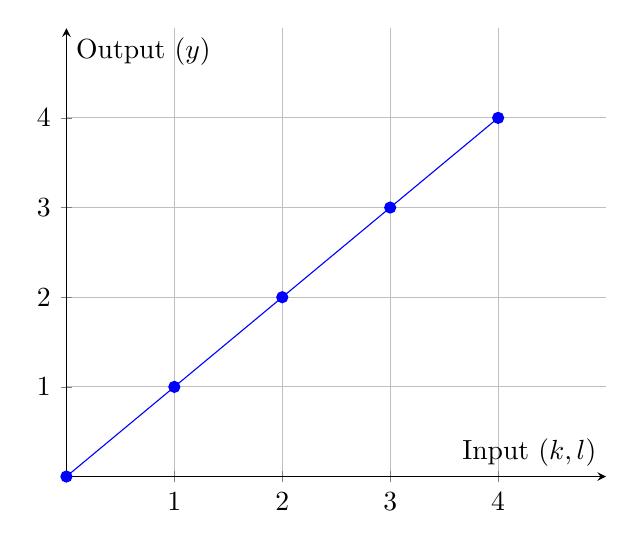
\begin{tikzpicture}
        \begin{axis}[
            axis lines = middle,
            xlabel = {Input ($k, l$)},
            ylabel = {Output ($y$)},
            xmin = 0, xmax = 5,
            ymin = 0, ymax = 5,
            xtick = {1, 2, 3, 4},
            ytick = {1, 2, 3, 4},
            grid = both,
        ]
        % Linear plot points
        \addplot[color=blue, mark=*] coordinates {
            (0,0)
            (1,1)
            (2,2)
            (3,3)
            (4,4)
        };
        \end{axis}
    \end{tikzpicture}
\end{center}
We see that the function exhibits return to scale constantly. 
\subsection*{d}
Let $\lambda \in \mathbb{R}$. We see that 
\[
A(\lambda L)^{0.5}(\lambda k)^{0.5} = \lambda A k L 
\]
which is directly proprotional to that of the function with no scaled inputs. Therefore, this function returns to scale mathematically. 
\subsection*{e}
If we double our inputs into a firm, they will produce exactly double the amount, which matches the logic of what we are presented in an ideal reality. 
\end{document}